\documentclass[crop,tikz]{standalone}

\usepackage[utf8]{inputenc}
\usepackage{ifthen}
\usepackage{amsmath}

% 'crop' is the default for v1.0, before it was 'preview'
%\usetikzlibrary{...}% tikz package already loaded by 'tikz' option

\begin{document}

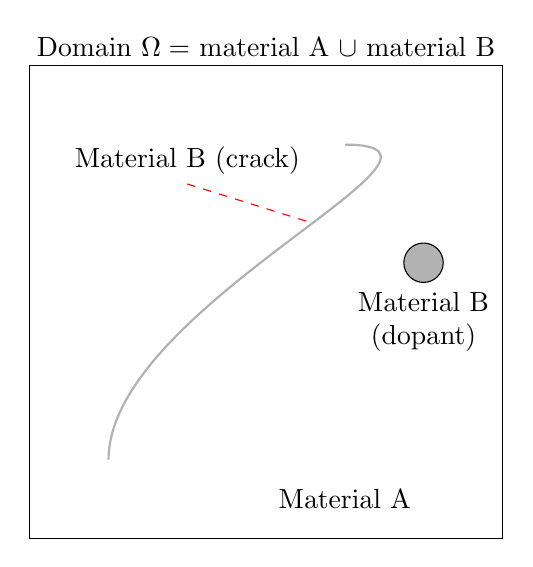
\begin{tikzpicture}

	\draw (-3,-3) rectangle (3,3);
	\draw[black!30!white, thick] (-2,-2) to[in=0, out=90] (1,2);
	
	\node at (1,-2.5) {Material A};
	\node[anchor=south] at (-1,1.5) {Material B (crack)};
	\draw[red, dashed] (-1,1.5) -- (0.6,1);
	
	\draw[fill=black!30!white] (2,0.5) circle (0.25);
	\node[anchor=north, align=center] at (2,0.25) {Material B \\ (dopant)};
	
	\node[anchor=south] at (0,3) {Domain $\Omega = $ material A $\cup$ material B};
		
\end{tikzpicture}

\end{document}